\documentclass{beamer}
%\hypersetup{pdfpagemode=FullScreen}
\usetheme{Luebeck}
\usepackage{CJKutf8}
\usepackage{graphicx}
\usepackage{setspace}


\title{Final Presentation}
\subtitle{Team 2}
\begin{document}

\begin{frame}
  \titlepage
\end{frame}

 \tableofcontents

\section{Producing presentation slides using the LaTex \medskip}
\begin{frame}{Producing presentation slides using the LaTex}
	(Fig.\,\ref{fig:1})
    \begin{figure}
  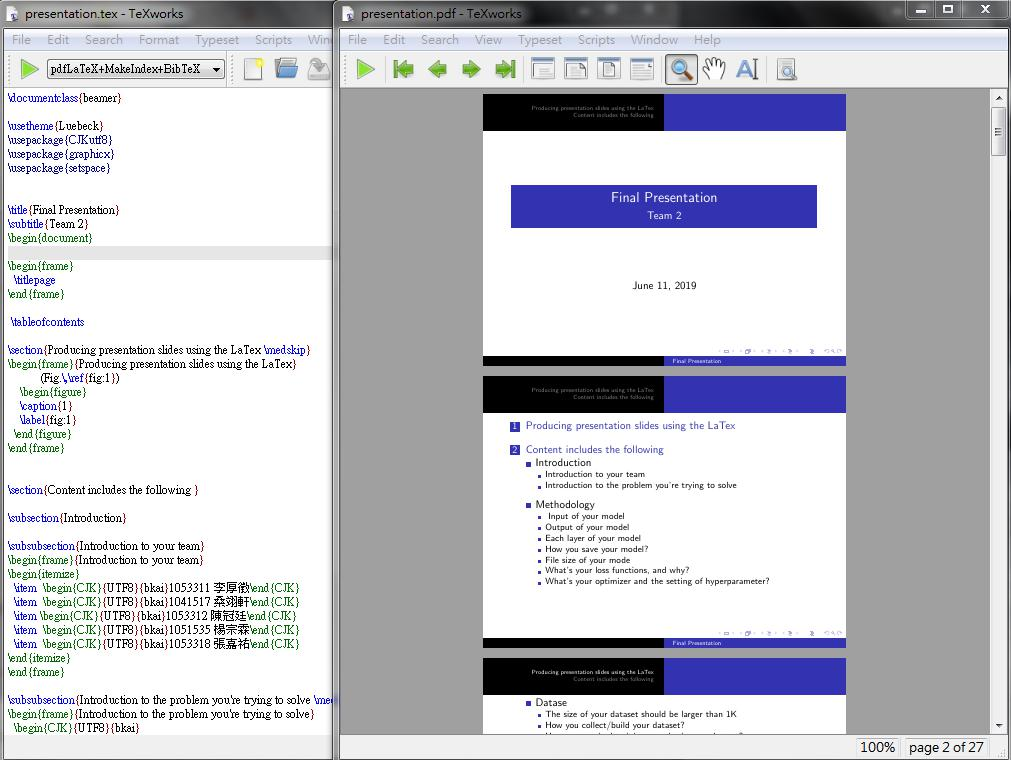
\includegraphics[width=0.7\linewidth]{latex.jpg}
    \caption{1}
    \label{fig:1}
  \end{figure}
\end{frame}


\section{Content includes the following }

\subsection{Introduction}

\begin{frame}{Introduction}
\center \huge Introduction
\end{frame} 


\subsubsection{Introduction to your team}
\begin{frame}{Our team members}
\begin{itemize}
\begin{CJK}{UTF8}{bkai}
  \item   1053311 李厚徵
  \item   1041517 桑翊軒
  \item   1053312 陳冠廷
  \item   1051535 楊宗霖
  \item   1053318 張嘉祐
\end{CJK}
\end{itemize}
\end{frame}

\subsubsection{Introduction to the problem you're trying to solve \medskip}
\begin{frame}{The problem we're trying to solve}
  \begin{CJK}{UTF8}{bkai}
      \begin{spacing}{1.5}\qquad
	期末專題主要是想解決我們對大自然的好奇心,
	當我們在校園探索當中,有很多花我們不知道其名稱,
	透過這門課所學的知識,利用影像辨識的方法,將各種花朵辨識出來。
	\end{spacing}
  \end{CJK}
\end{frame}

\subsection{Methodology}
\begin{frame}{Methodology}
\center \huge Methodology
\end{frame}

\subsubsection{Input of your model }
\begin{frame}{Model}
  input of our model (Fig.\,\ref{fig:2})
    \begin{figure}
   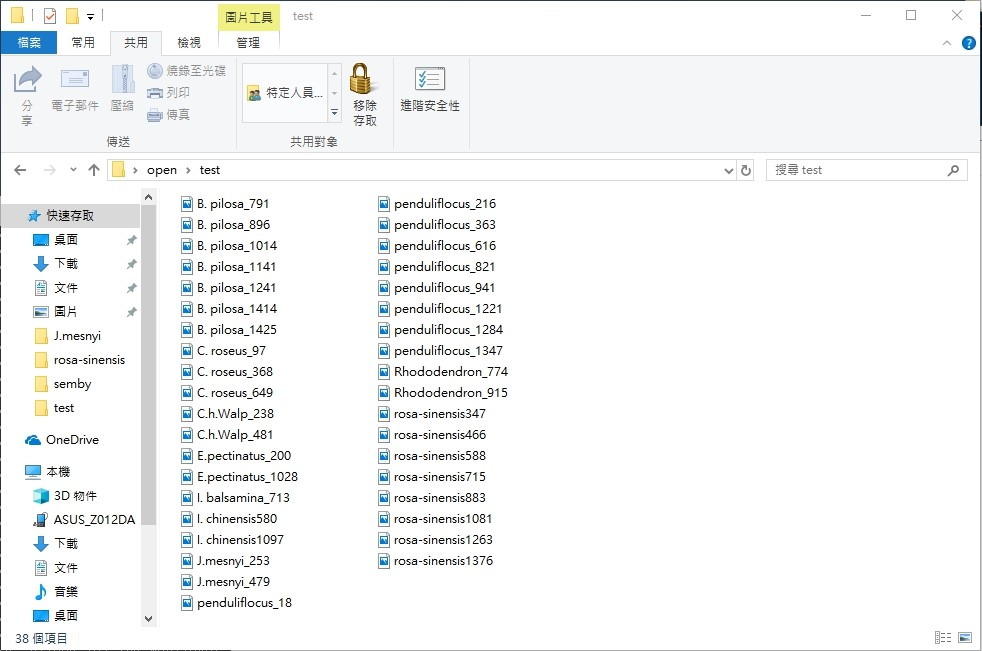
\includegraphics[width=0.7\linewidth]{input.jpg}
    \caption{2}
    \label{fig:2}
  \end{figure}
\end{frame}

\subsubsection{Output of your model}
\begin{frame}{Model(cont.)}
  \begin{CJK}{UTF8}{bkai}
output of our model , prediction result(包含: 預測的label, 其信心度)(Fig.\,\ref{fig:3})
  \end{CJK}
    \begin{figure}
      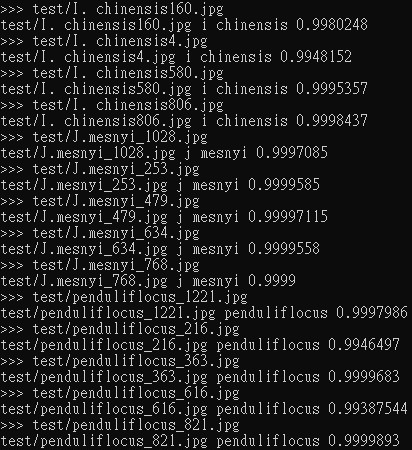
\includegraphics[width=7cm,height=5cm]{output(1).jpg}
      \caption{3}
      \label{fig:3}
    \end{figure}
\end{frame}

\begin{frame}{Model(cont.)}
  \begin{CJK}{UTF8}{bkai}
(Fig.\,\ref{fig:4})
  \end{CJK}
    \begin{figure}
      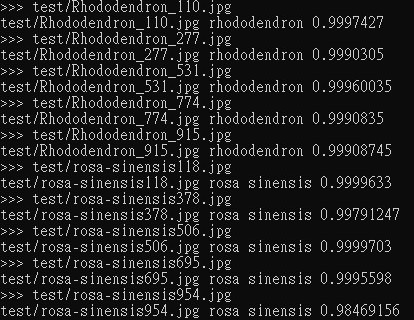
\includegraphics[width=7cm,height=6cm]{output(2).jpg}
      \caption{4}
      \label{fig:4}
    \end{figure}
\end{frame}

\subsubsection{Each layer of your model }
\begin{frame}{Model(cont.)}
 \begin{CJK}{UTF8}{bkai}
 我們的model層級分成: Expansion layer, convolution layer, projection layer… (Fig.\,\ref{fig:5})
\end{CJK}
  \begin{figure}
    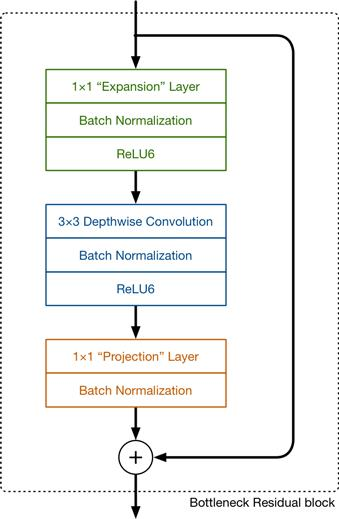
\includegraphics[width=0.3\linewidth]{layer.jpg}
    \caption{5}
    \label{fig:5}
  \end{figure}
\end{frame}

\subsubsection{How you save your model? }
\begin{frame}{Model(cont.)}
  \begin{CJK}{UTF8}{bkai}
	We save as filename.pb(pb檔)
   \end{CJK}
  \begin{figure}
      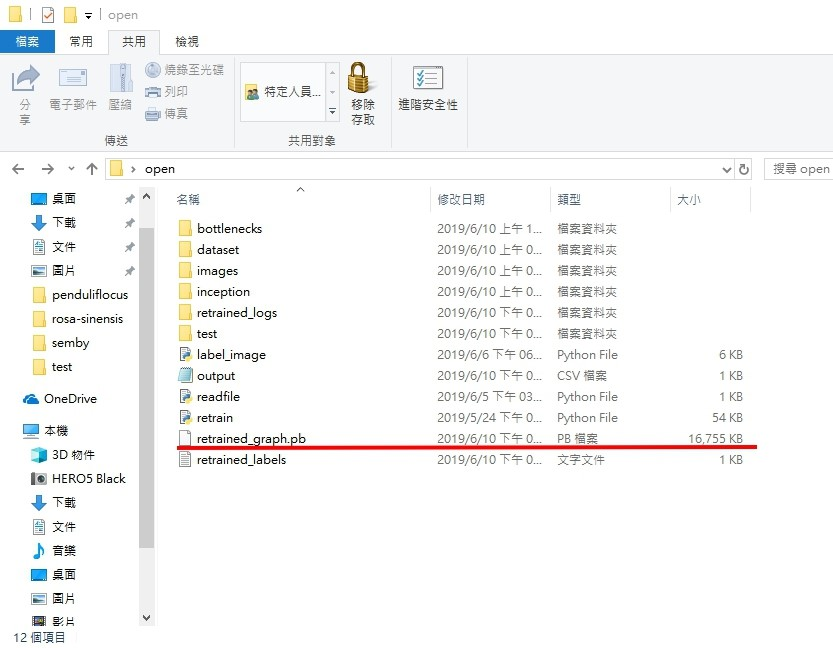
\includegraphics[width=0.6\linewidth]{pbfile.jpg}(Fig.\,\ref{fig:6})
      \caption{6}
      \label{fig:6}
    \end{figure}
\end{frame}

\subsubsection{File size of your model }
\begin{frame}{Model(cont.)}
 \begin{figure}
 \begin{CJK}{UTF8}{bkai}
   model大小16755KB   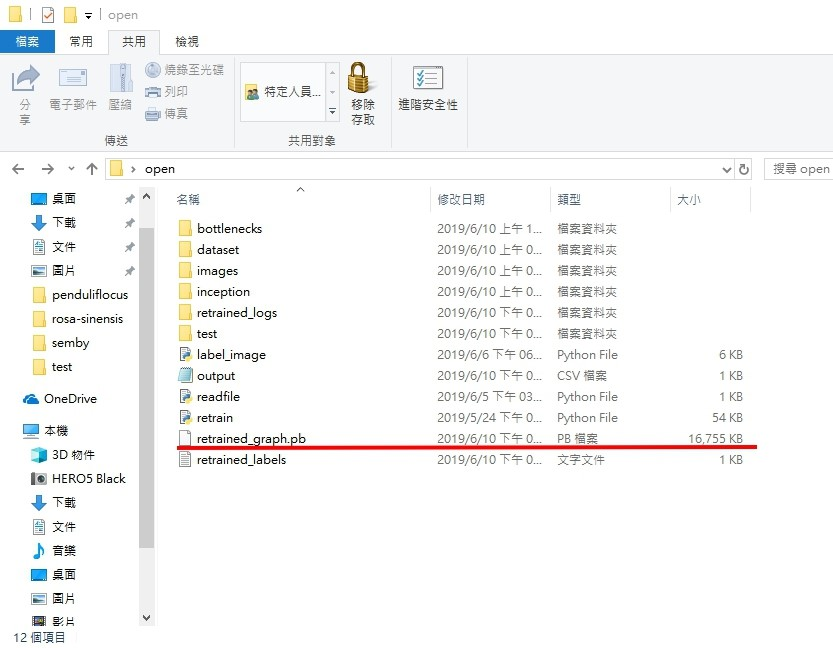
\includegraphics[width=0.65\linewidth]{pbfile.jpg}(Fig.\,\ref{fig:7})
  \end{CJK}
      \caption{7}
      \label{fig:7}
    \end{figure}
\end{frame}

\subsubsection{What's your loss functions, and why? \bigskip \bigskip \bigskip  \bigskip  \bigskip   }
\begin{frame}{Loss function}
  \begin{CJK}{UTF8}{bkai}
	Cross-entropy:\\
	在分類的狀況下,通常希望錯誤率越小越好,所以用錯誤率當損失函數是一個選項,但實際上我們並不會直接拿分類錯誤率當作損失函數進行最佳化,
	用錯誤率得到只知道此筆資料判別錯誤,但模型不會知道現在的模型錯的很多還是很少,
	這樣模型在學習時根本不知道最佳的模型在那的方向,也不知道要更新多少。
	\\
	Cross-entropy 是 所有類別的entropy的總和,簡單來說,
	就是各類別的訊息量的平均量(entropy)的總和。entropy也可以解釋成資料的不確定性,
	所以越低代表資料越穩定也就是說model越好。
   \end{CJK}
\end{frame}





\subsection{Dataset}
\subsubsection{The size of your dataset should be larger than 1K}

\begin{frame}{Dataset}

\center \huge Dataset
\end{frame}

\begin{frame}{Dataset}
  \begin{CJK}{UTF8}{bkai}
The size of our dataset  大小4.85GB 共有11098個檔案 (Fig.\,\ref{fig:8})
   \end{CJK}
 \begin{figure}
    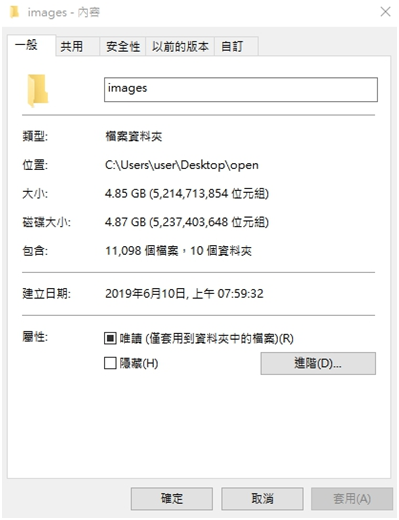
\includegraphics[width=5cm,height=5cm]{dataset(1).png}
    \caption{8}
    \label{fig:8}
  \end{figure}

\end{frame}


\begin{frame}{Dataset(cont.)}
 \begin{CJK}{UTF8}{bkai}
dataset 檔案 (Fig.\,\ref{fig:9})
 \begin{figure}
    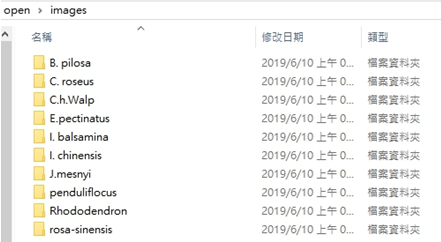
\includegraphics[width=8cm]{dataset(2).png}
    \caption{9}
    \label{fig:9}
  \end{figure}
  \end{CJK}
\end{frame}

\subsubsection{How you collect/build your dataset?}
\begin{frame}{Dataset(cont.)}
  \begin{CJK}{UTF8}{bkai}
	dataset的收集方法我們是對花做360度的影片拍攝,再將影片以frame切割得到圖片。\\
           \bigskip
   	training、validating以及testing的配對樣本數比例是:
	training:validating:testing = 8:1:1
   \end{CJK}
\end{frame}

\subsubsection{How many paired training samples in your dataset?}


\subsubsection{How many paired validating samples in your dataset?}


\subsubsection{How many paired testing samples in your dataset?}


\subsection{Experimental Evaluation }
\begin{frame}{Experimental Evaluation}
\center \huge Experimental Evaluation
\end{frame}

\subsubsection{Experimental environment (CPU, GPU, memory,…,etc.)}
\begin{frame}{Experimental Evaluation}
 \begin{CJK}{UTF8}{bkai}
我們是在CPU的環境下進行實作及試驗\\ \bigskip
設定4000 ephocs 來進行訓練
\end{CJK}
\end{frame}

\subsubsection{How many epochs you set for training?}


\subsubsection{Qualitative evaluation}
\begin{frame}{Qualitative}
\begin{CJK}{UTF8}{bkai}
\small 共10種花,對每種花各做五次測試的結果 共50個測資皆正確。(Fig.\,\ref{fig:10})
 \end{CJK}
 \begin{figure}
    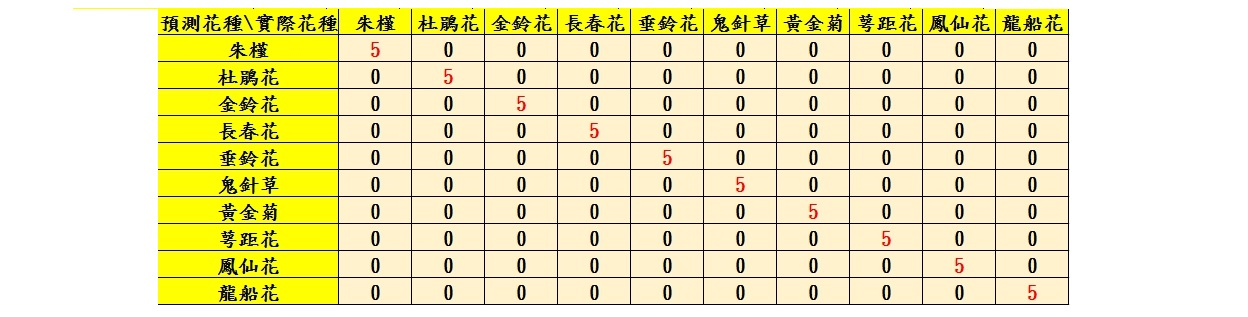
\includegraphics[width=12cm,height=5cm]{qualitative.jpg}
    \caption{10}
    \label{fig:10}
  \end{figure}
\end{frame}




\subsubsection{Quantitative evaluation}
\begin{frame}{Quantitative}

\begin{CJK}{UTF8}{bkai}
(Fig.\,\ref{fig:14})  
以下是實作的結果值
 \end{CJK}
 \begin{figure}
    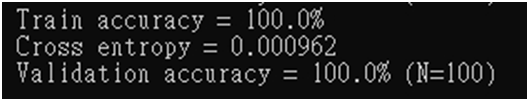
\includegraphics[width=10cm]{Qauntitative.png}
    \caption{14}
    \label{fig:14}
  \end{figure}


\end{frame}

\subsection{Live demo of your work}

\begin{frame}
\center \huge End
\end{frame}

\end{document}